\documentclass{standalone}
\usepackage{tikz}
\usetikzlibrary{patterns, positioning}

\begin{document}
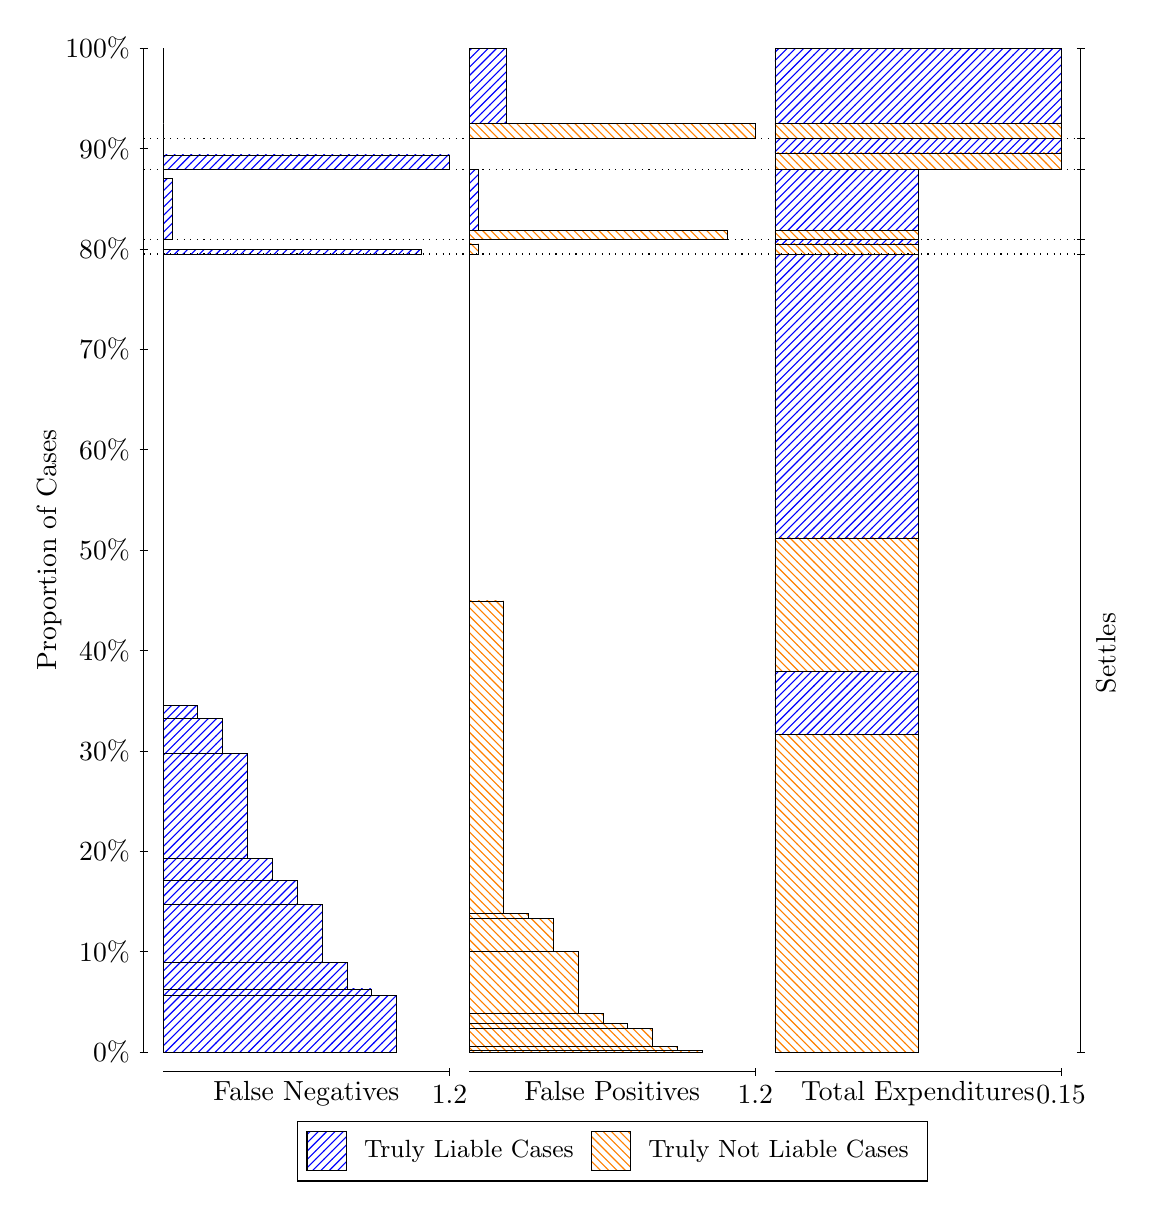
\begin{tikzpicture}
\draw[black, very thin] (1.5,1.75) -- (1.5,14.5);
\node[rotate=90, anchor=center] at (0.3, 8.125) {Proportion of Cases};
\draw[black, very thin] (1.45,1.75) -- (1.55,1.75);
\node[anchor=east] at (1.45, 1.75) {0\%};
\draw[black, very thin] (1.45,3.025) -- (1.55,3.025);
\node[anchor=east] at (1.45, 3.025) {10\%};
\draw[black, very thin] (1.45,4.3) -- (1.55,4.3);
\node[anchor=east] at (1.45, 4.3) {20\%};
\draw[black, very thin] (1.45,5.575) -- (1.55,5.575);
\node[anchor=east] at (1.45, 5.575) {30\%};
\draw[black, very thin] (1.45,6.85) -- (1.55,6.85);
\node[anchor=east] at (1.45, 6.85) {40\%};
\draw[black, very thin] (1.45,8.125) -- (1.55,8.125);
\node[anchor=east] at (1.45, 8.125) {50\%};
\draw[black, very thin] (1.45,9.4) -- (1.55,9.4);
\node[anchor=east] at (1.45, 9.4) {60\%};
\draw[black, very thin] (1.45,10.675) -- (1.55,10.675);
\node[anchor=east] at (1.45, 10.675) {70\%};
\draw[black, very thin] (1.45,11.95) -- (1.55,11.95);
\node[anchor=east] at (1.45, 11.95) {80\%};
\draw[black, very thin] (1.45,13.225) -- (1.55,13.225);
\node[anchor=east] at (1.45, 13.225) {90\%};
\draw[black, very thin] (1.45,14.5) -- (1.55,14.5);
\node[anchor=east] at (1.45, 14.5) {100\%};

\draw[black, very thin] (13.4,1.75) -- (13.4,14.5);
\draw[black, very thin] (13.35,1.75) -- (13.45,1.75);
\node[anchor=west] at (13.35, 1.75) {};
\draw[black, very thin] (13.35,11.884) -- (13.45,11.884);
\node[anchor=west] at (13.35, 11.884) {};
\draw[black, very thin] (13.35,12.07) -- (13.45,12.07);
\node[anchor=west] at (13.35, 12.07) {};
\draw[black, very thin] (13.35,12.958) -- (13.45,12.958);
\node[anchor=west] at (13.35, 12.958) {};
\draw[black, very thin] (13.35,13.353) -- (13.45,13.353);
\node[anchor=west] at (13.35, 13.353) {};
\draw[black, very thin] (13.35,14.5) -- (13.45,14.5);
\node[anchor=west] at (13.35, 14.5) {};

\draw[black, very thin, pattern color=blue, pattern=north east lines] (1.75,1.75) rectangle (4.712,2.4676);
\draw[black, very thin, pattern color=blue, pattern=north east lines] (1.75,2.4676) rectangle (4.396,2.5516);
\draw[black, very thin, pattern color=blue, pattern=north east lines] (1.75,2.5516) rectangle (4.0801,2.8908);
\draw[black, very thin, pattern color=blue, pattern=north east lines] (1.75,2.8908) rectangle (3.7641,3.6246);
\draw[black, very thin, pattern color=blue, pattern=north east lines] (1.75,3.6246) rectangle (3.4482,3.9249);
\draw[black, very thin, pattern color=blue, pattern=north east lines] (1.75,3.9249) rectangle (3.1322,4.205);
\draw[black, very thin, pattern color=blue, pattern=north east lines] (1.75,4.205) rectangle (2.8163,5.5389);
\draw[black, very thin, pattern color=blue, pattern=north east lines] (1.75,5.5389) rectangle (2.5004,5.9912);
\draw[black, very thin, pattern color=blue, pattern=north east lines] (1.75,5.9912) rectangle (2.1844,6.1558);
\draw[black, very thin, pattern color=orange, pattern=north west lines] (1.75,6.1558) rectangle (1.75,11.884);
\draw[black, very thin, pattern color=blue, pattern=north east lines] (1.75,11.884) rectangle (5.0279,11.94);
\draw[black, very thin, pattern color=orange, pattern=north west lines] (1.75,11.94) rectangle (1.75,12.07);
\draw[black, very thin, pattern color=blue, pattern=north east lines] (1.75,12.07) rectangle (1.8685,12.84);
\draw[black, very thin, pattern color=orange, pattern=north west lines] (1.75,12.84) rectangle (1.75,12.958);
\draw[black, very thin, pattern color=blue, pattern=north east lines] (1.75,12.958) rectangle (5.3833,13.144);
\draw[black, very thin, pattern color=orange, pattern=north west lines] (1.75,13.144) rectangle (1.75,13.353);
\draw[black, very thin, pattern color=orange, pattern=north west lines] (1.75,13.353) rectangle (1.75,13.543);
\draw[black, very thin, pattern color=blue, pattern=north east lines] (1.75,13.543) rectangle (1.75,14.5);
\draw[black, very thin, pattern color=orange, pattern=north west lines] (5.6333,1.75) rectangle (8.5953,1.7672);
\draw[black, very thin, pattern color=orange, pattern=north west lines] (5.6333,1.7672) rectangle (8.2793,1.8176);
\draw[black, very thin, pattern color=orange, pattern=north west lines] (5.6333,1.8176) rectangle (7.9634,2.0448);
\draw[black, very thin, pattern color=orange, pattern=north west lines] (5.6333,2.0448) rectangle (7.6475,2.1089);
\draw[black, very thin, pattern color=orange, pattern=north west lines] (5.6333,2.1089) rectangle (7.3315,2.2417);
\draw[black, very thin, pattern color=orange, pattern=north west lines] (5.6333,2.2417) rectangle (7.0156,2.2465);
\draw[black, very thin, pattern color=orange, pattern=north west lines] (5.6333,2.2465) rectangle (7.0156,3.0303);
\draw[black, very thin, pattern color=orange, pattern=north west lines] (5.6333,3.0303) rectangle (6.6996,3.4454);
\draw[black, very thin, pattern color=orange, pattern=north west lines] (5.6333,3.4454) rectangle (6.3837,3.5081);
\draw[black, very thin, pattern color=orange, pattern=north west lines] (5.6333,3.5081) rectangle (6.0678,7.4782);
\draw[black, very thin, pattern color=blue, pattern=north east lines] (5.6333,7.4782) rectangle (5.6333,11.884);
\draw[black, very thin, pattern color=orange, pattern=north west lines] (5.6333,11.884) rectangle (5.7518,12.014);
\draw[black, very thin, pattern color=blue, pattern=north east lines] (5.6333,12.014) rectangle (5.6333,12.07);
\draw[black, very thin, pattern color=orange, pattern=north west lines] (5.6333,12.07) rectangle (8.9112,12.188);
\draw[black, very thin, pattern color=blue, pattern=north east lines] (5.6333,12.188) rectangle (5.7518,12.958);
\draw[black, very thin, pattern color=orange, pattern=north west lines] (5.6333,12.958) rectangle (5.6333,13.167);
\draw[black, very thin, pattern color=blue, pattern=north east lines] (5.6333,13.167) rectangle (5.6333,13.353);
\draw[black, very thin, pattern color=orange, pattern=north west lines] (5.6333,13.353) rectangle (9.2667,13.543);
\draw[black, very thin, pattern color=blue, pattern=north east lines] (5.6333,13.543) rectangle (6.1072,14.5);
\draw[black, very thin, pattern color=orange, pattern=north west lines] (9.5167,1.75) rectangle (11.333,5.7827);
\draw[black, very thin, pattern color=blue, pattern=north east lines] (9.5167,5.7827) rectangle (11.333,6.5843);
\draw[black, very thin, pattern color=orange, pattern=north west lines] (9.5167,6.5843) rectangle (11.333,8.2798);
\draw[black, very thin, pattern color=blue, pattern=north east lines] (9.5167,8.2798) rectangle (11.333,11.884);
\draw[black, very thin, pattern color=orange, pattern=north west lines] (9.5167,11.884) rectangle (11.333,12.014);
\draw[black, very thin, pattern color=blue, pattern=north east lines] (9.5167,12.014) rectangle (11.333,12.07);
\draw[black, very thin, pattern color=orange, pattern=north west lines] (9.5167,12.07) rectangle (11.333,12.188);
\draw[black, very thin, pattern color=blue, pattern=north east lines] (9.5167,12.188) rectangle (11.333,12.958);
\draw[black, very thin, pattern color=orange, pattern=north west lines] (9.5167,12.958) rectangle (13.15,13.167);
\draw[black, very thin, pattern color=blue, pattern=north east lines] (9.5167,13.167) rectangle (13.15,13.353);
\draw[black, very thin, pattern color=orange, pattern=north west lines] (9.5167,13.353) rectangle (13.15,13.543);
\draw[black, very thin, pattern color=blue, pattern=north east lines] (9.5167,13.543) rectangle (13.15,14.5);
\draw[black, dotted] (1.5,11.884) -- (13.4,11.884);
\draw[black, dotted] (1.5,12.07) -- (13.4,12.07);
\draw[black, dotted] (1.5,12.958) -- (13.4,12.958);
\draw[black, dotted] (1.5,13.353) -- (13.4,13.353);
\draw[black, very thin] (1.75,1.5) -- (5.3833,1.5);
\node[anchor=north] at (3.5667, 1.5) {False Negatives};
\draw[black, very thin] (5.3833,1.45) -- (5.3833,1.55);
\node[anchor=north] at (5.3833, 1.45) {1.2};

\draw[black, very thin] (5.6333,1.5) -- (9.2667,1.5);
\node[anchor=north] at (7.45, 1.5) {False Positives};
\draw[black, very thin] (9.2667,1.45) -- (9.2667,1.55);
\node[anchor=north] at (9.2667, 1.45) {1.2};

\draw[black, very thin] (9.5167,1.5) -- (13.15,1.5);
\node[anchor=north] at (11.333, 1.5) {Total Expenditures};
\draw[black, very thin] (13.15,1.45) -- (13.15,1.55);
\node[anchor=north] at (13.15, 1.45) {0.15};

\node[black, centered, rotate=90] at (13.72, 6.817) {Settles};





\draw (7.449999999999999,1.5) node[draw=none] (baseCoordinate) {};
\begin{scope}[align=center]
        \matrix[scale=0.5, draw=black, below=0.5cm of baseCoordinate, nodes={draw}, column sep=0.1cm]{
            \node[rectangle, draw, minimum width=0.5cm, minimum height=0.5cm, pattern=north east lines, pattern color=blue] {}; &
            \node[draw=none, font=\small] (B) {Truly Liable Cases}; &
            \node[rectangle, draw, minimum width=0.5cm, minimum height=0.5cm, pattern=north west lines, pattern color=orange] {}; &
            \node[draw=none, font=\small] (B) {Truly Not Liable Cases}; \\
            };
\end{scope}

\end{tikzpicture}
\end{document}